\documentclass[border=4pt,12pt]{standalone}
% House style for redrawn exam diagrams (diagram-v4: 0.4pt lines, filled -latex arrows, fine dashes; stipple and hatching drawn as real dots/lines (no PDF/SVG patterns, so they render in every browser and at any scale); transparent background). Every figure \input's this.
\usepackage{amsmath,amssymb}
\usepackage{txfonts}
\usepackage{pdfrender,xcolor}
% \halo{text}: label on shading. The shading stops just around each letter's outline (a thin knock-out that follows the
% glyphs, like the papers' typesetting), never a box. Owner: "I don't want a box around the text".
\newcommand{\halo}[1]{\leavevmode\rlap{\pdfrender{TextRenderingMode=2,LineWidth=2.2pt,LineJoinStyle=1,StrokeColor=white,FillColor=white}#1}#1}
\usepackage{tikz,pgfplots}
\pgfplotsset{compat=1.18}
\usetikzlibrary{arrows.meta,calc,angles,quotes,patterns,patterns.meta,intersections,positioning,decorations.markings,shapes.geometric}
% Stipple and hatching are drawn as actual dots / lines clipped to the region (path picture), NOT as pattern fills:
% SVG <pattern> fills vanish or blur when browsers scale the image, so the owner could not see the shading.
% Each dot is a 0.72pt square (keeps SVGs small; reads as a dot at print size). Dots sit on one global staggered grid, so neighbouring regions line up.
\makeatletter
\newdimen\ex@x \newdimen\ex@y \newdimen\ex@xa \newdimen\ex@ya \newdimen\ex@xb \newdimen\ex@yb \newcount\ex@row
\def\exam@stipplecolor{black!75}\def\exam@dotr{0.42pt}\def\exam@dotgap{2.5}
\def\ex@rowdots{\ifdim\ex@x<\ex@xb \pgfpathrectangle{\pgfqpoint{\dimexpr\ex@x-0.36pt\relax}{\dimexpr\ex@y-0.36pt\relax}}{\pgfqpoint{0.72pt}{0.72pt}}\advance\ex@x by \exam@dotgap pt\relax\expandafter\ex@rowdots\fi}
\def\exam@stipple{%
  \pgftransformreset% dots are sized in real points even inside scaled pictures
  \pgfpointanchor{path picture bounding box}{south west}\ex@xa=\pgf@x \ex@ya=\pgf@y
  \pgfpointanchor{path picture bounding box}{north east}\ex@xb=\pgf@x \ex@yb=\pgf@y
  \pgfsetfillcolor{\exam@stipplecolor}\pgfmathsetmacro\ex@h{\exam@dotgap/2}%
  \pgfmathtruncatemacro\ex@r{floor(\ex@ya/\ex@h)-1}\ex@row=\ex@r\relax
  \ex@y=\ex@r\dimexpr\ex@h pt\relax
  \loop\ifdim\ex@y<\ex@yb
    \pgfmathtruncatemacro\ex@c{floor(\ex@xa/\exam@dotgap)-1}\ex@x=\ex@c\dimexpr\exam@dotgap pt\relax
    \ifodd\ex@row \advance\ex@x by \ex@h pt\fi
    \ex@rowdots
    \advance\ex@y by \ex@h pt \advance\ex@row by 1
    \ifnum\numexpr\ex@row-(\ex@row/4)*4\relax=0 \pgfusepath{fill}\fi% flush every 4 rows: bounded TeX memory, few clip copies in the SVG
  \repeat\pgfusepath{fill}}
\newdimen\ex@d
\def\exam@hatch#1{% #1 = 1 for /, -1 for \ ; lines 45 degrees, 3pt apart
  \pgftransformreset
  \pgfpointanchor{path picture bounding box}{south west}\ex@xa=\pgf@x \ex@ya=\pgf@y
  \pgfpointanchor{path picture bounding box}{north east}\ex@xb=\pgf@x \ex@yb=\pgf@y
  \ex@d=\dimexpr\ex@yb-\ex@ya\relax \ex@x=\dimexpr\ex@xa-\ex@d\relax
  \loop\ifdim\ex@x<\ex@xb
    \ifnum#1>0 \pgfpathmoveto{\pgfqpoint{\ex@x}{\ex@ya}}\pgfpathlineto{\pgfqpoint{\dimexpr\ex@x+\ex@d\relax}{\ex@yb}}%
    \else \pgfpathmoveto{\pgfqpoint{\ex@x}{\ex@yb}}\pgfpathlineto{\pgfqpoint{\dimexpr\ex@x+\ex@d\relax}{\ex@ya}}\fi
    \advance\ex@x by 4.24pt
  \repeat
  \pgfsetlinewidth{0.4pt}\pgfsetstrokecolor{black}\pgfusepath{stroke}}
\def\examstipple{\exam@stipple}\def\examhatch{\exam@hatch}\def\examsetstipplecolor#1{\def\exam@stipplecolor{#1}}\def\examsetdotgap#1{\def\exam@dotgap{#1}}
\makeatother
% (legacy pattern kept for old files)
% staggered stipple like the NESA papers' dotted shading
\pgfdeclarepatternformonly{exam stipple}{\pgfpointorigin}{\pgfqpoint{2.2pt}{2.2pt}}{\pgfqpoint{2.2pt}{2.2pt}}{%
  \pgfpathcircle{\pgfqpoint{0.55pt}{0.55pt}}{0.42pt}\pgfpathcircle{\pgfqpoint{1.65pt}{1.65pt}}{0.42pt}\pgfusepath{fill}}
\tikzset{
  every picture/.style={line width=0.6pt, >={Latex[length=2mm,width=1.3mm]}},
  curve/.style={line width=0.6pt},
  open arrow/.style={-{Latex[length=2mm,width=1.3mm]}},  % owner: filled -latex heads everywhere, no open chevrons
  aux/.style={dash pattern=on 2pt off 1.5pt, line width=0.6pt},
  shade/.code={\def\exA{#1}\def\exB{none}\ifx\exA\exB\else\pgfkeysalso{fill=black!18}\fi},
  shade/.default=on,
  shade dots/.style={fill=none, path picture={\examstipple}},
  stipple color/.code={\examsetstipplecolor{#1}},
  stipple gap/.code={\examsetdotgap{#1}},
  shade dense dots/.style={fill=none, stipple gap=1.6, path picture={\examstipple}},
  shade hatch/.style={fill=none, path picture={\examhatch{1}}},
  shade hatch reverse/.style={fill=none, path picture={\examhatch{-1}}},
  shade solid/.style={fill=black},
  pt/.style={circle, fill, inner sep=1.1pt},
  open pt/.style={circle, draw, fill=white, inner sep=1.1pt},
}
\pgfplotsset{
  exam axes/.style={axis lines=middle, axis line style={->}, xlabel={$x$}, ylabel={$y$},
    xlabel style={anchor=west}, ylabel style={anchor=south}, tick label style={font=\small},
    every axis plot/.append style={line width=0.6pt, black}, samples=200, clip=false,
    enlargelimits=false, axis on top},
}

\begin{document}
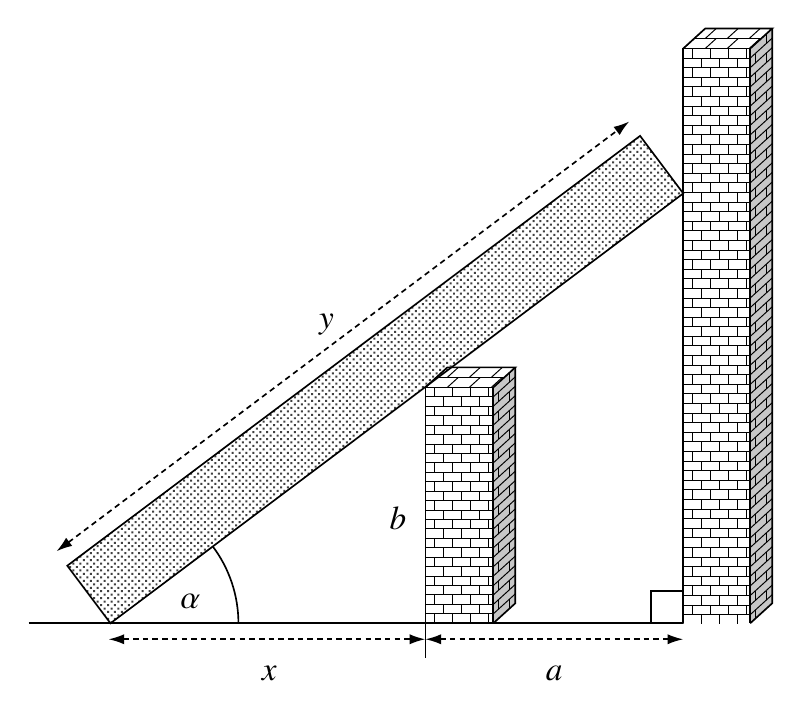
\begin{tikzpicture}[x=0.0127cm,y=-0.0127cm]
\tikzset{brick/.style={line width=0.35pt}}
\newcommand\wall[5]{% #1 x0, #2 x1, #3 ytop, #4 courses, #5 course height; depth vector (22,-20)
  \begin{scope}
    \clip (#1,#3) rectangle (#2,610);
    \foreach \k in {1,...,#4} {
      \pgfmathsetmacro\yy{#3+(\k-1)*#5}
      \draw[brick] (#1,\yy) -- (#2,\yy);
      \pgfmathsetmacro\off{mod(\k,2)*9}
      \foreach \j in {0,...,4} \draw[brick] ({#1+\off+\j*18},\yy) -- ({#1+\off+\j*18},{\yy+#5});
    }
  \end{scope}
  \fill[black!22] (#2,#3) -- ++(22,-20) -- (#2+22,590) -- (#2,610) -- cycle;
  \begin{scope}
    \clip (#2,#3) -- ++(22,-20) -- (#2+22,590) -- (#2,610) -- cycle;
    \foreach \k in {1,...,#4} {
      \pgfmathsetmacro\yy{#3+(\k-1)*#5}
      \draw[brick] (#2,\yy) -- ++(22,-20);
      \pgfmathsetmacro\off{mod(\k,2)*11}
      \draw[brick] ({#2+5+\off},{\yy-(5+\off)*20/22}) -- ++(0,#5);
    }
  \end{scope}
  \begin{scope}
    \clip (#1,#3) -- ++(22,-20) -- (#2+22,#3-20) -- (#2,#3) -- cycle;
    \draw[brick] (#1+11,#3-10) -- (#2+11,#3-10);
    \foreach \j in {0,...,3} {
      \draw[brick] ({#1+\j*22},#3) -- ++(11,-10);
      \draw[brick] ({#1+22+\j*22},#3-10) -- ++(11,-10);
    }
  \end{scope}
  \draw (#1,610) -- (#1,#3) -- (#2,#3) -- (#2,610);
  \draw (#1,#3) -- ++(22,-20) -- (#2+22,#3-20) -- (#2,#3);
  \draw (#2+22,#3-20) -- (#2+22,590) -- (#2,610);
}
\wall{397}{465}{374}{25}{9.44}
\wall{655}{722}{35}{60}{9.6}
\draw (0,610) -- (655,610);
\draw (623,610) -- (623,578) -- (655,578);
\path[shade dots] (82,610) -- (655,180) -- (611.8,122.4) -- (38.8,552.4) -- cycle;
\draw (82,610) -- (655,180) -- (611.8,122.4) -- (38.8,552.4) -- cycle;
\draw (210,610) arc[start angle=0,end angle=-36.87,radius=128];
\node[font=\large] at (162,588) {$\alpha$};
\draw[aux,<->] ($(38.8,552.4)+(-10.8,-14.4)$) -- ($(611.8,122.4)+(-10.8,-14.4)$);
\node[font=\large] at (298,311) {$y$};
\draw[line width=0.4pt] (397,610) -- (397,645);
\draw[aux,<->] (80,626) -- (397,626);
\draw[aux,<->] (397,626) -- (655,626);
\node[font=\large] at (240,660) {$x$};
\node[font=\large] at (526,660) {$a$};
\node[font=\large,anchor=east] at (388,505) {$b$};
\end{tikzpicture}
\end{document}